\documentclass{beamer}

\usepackage[utf8]{inputenc}
\usepackage{default}

\usetheme{Warsaw}



\begin{document}
\title{Numerical Relation Extraction}  
\author{Aman Madaan, Ashish Mittal}
\date{\today}

\begin{frame}
\frametitle{Introduction}

\begin{itemize}
 
 \item  Wealth of information is stored in unstructured text on the web.
 
  \begin{figure}
    \centering
    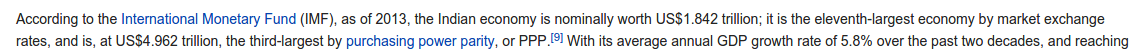
\includegraphics[width = 1.0\textwidth]{images/ex_1}
  \end{figure}
  
  \begin{figure}
    \centering
    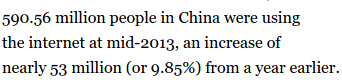
\includegraphics[width = 0.3\textwidth]{images/ex_2}
  \end{figure}
  
    \begin{figure}
    \centering
    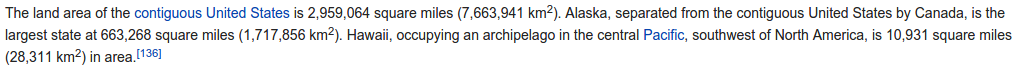
\includegraphics[width = 1.0\textwidth]{images/ex_3}
  \end{figure}
  

  \item Our focus is to extract the facts which are expressed in text using natural langauges and 
  create a database of such facts.
 
\end{itemize}

\end{frame}

\begin{frame}
 
 \frametitle{Relation Extraction Problem}
 
 \begin{itemize}
 \item The idea is that a number and an entity are related with some relation in a sentence.
 
 \item Our goal is to extract 3-tuples which consists of an entity and a numerical value that are bound by some relation.
  
    \begin{itemize}
	\item  (India, \textbf{economy}, 1.842 trillion USD)
	\item  (China, \textbf{internet users},  590.56 million)
	\item  (USA, \textbf{land area}, 2,959,054 square mile)
    \end{itemize}

 \end{itemize}

\end{frame}

\begin{frame}
 
 \frametitle{Why to use Machine Learning for Relation Extraction}
 
 \begin{itemize}
  
  \item  Structure and content of sentences expressing the same relations are expected to be similar. \pause
    
    \begin{itemize}
      \item The population of Australia is estimated to be 23,622,400 as of 7 October 2014.
      \item According to an official estimate for 1 June 2014, the population of Russia is 143,800,000. 
      
      
    \end{itemize}
      
    
 \end{itemize}
\end{frame}

\begin{frame}
 
 \frametitle{Why to use Machine Learning for Relation Extraction}
 
 \begin{itemize}
  
  \item  Structure and content of sentences expressing the same relations are expected to be similar. 
    
    \begin{itemize}   
	
      \item At 17,075,400 square kilometres, Russia is the largest country in the world.
      \item With an area of 504,030 $km^{2}$, Spain is the second largest country in Western Europe.
      
    \end{itemize}
 \end{itemize}
\end{frame}


\begin{frame}
 \frametitle{Why to use Machine Learning for Relation Extraction}
 
 \begin{itemize}
  \item Redundancy in grammatical features and dependencies of the sentences expressing same relation. \pause
     \begin{figure}
    \centering
    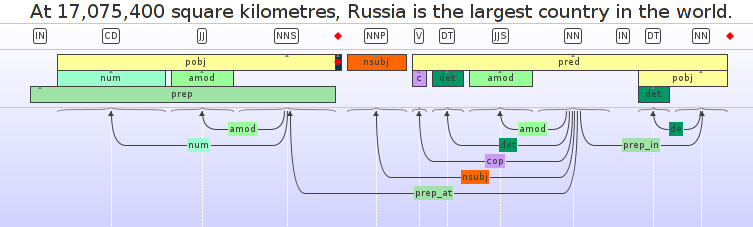
\includegraphics[width = 0.8\textwidth]{images/ex_4}
  \end{figure} \pause
  
   \begin{figure}
    \centering
    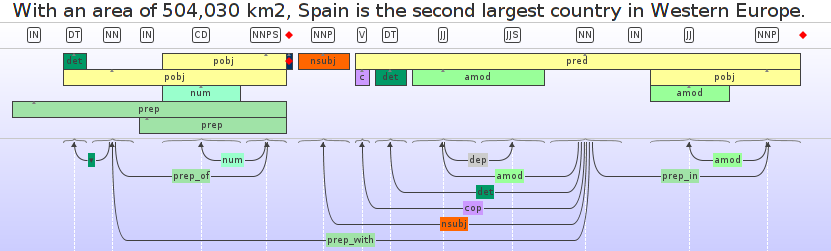
\includegraphics[width = 0.8\textwidth]{images/ex_5}
  \end{figure}
  
  
 \end{itemize}

\end{frame}

\begin{frame}
\frametitle{How to use Machine Learning for Relation Extraction}
\begin{itemize}
  \item There is lot of redundancy in ways in which a relation is expressed in sentence. \pause
  \item So for every relation learn the patterns that express it. \pause
    \begin{itemize}
      \item grammatical patterns - POS tags, dependency parse. \pause
      \item keywords for the relations. \pause
    \end{itemize}
    
    \item This forms the relation extraction as a multi-class classification problem.
 \end{itemize}
\end{frame}


\begin{frame}
 \frametitle{Relation Extraction Problem}
 
  \begin{itemize}
   \item Collect enough examples for each relation so that there are sufficient patterns and enough redundancy to exploit.
   \item Extract features (important keywords, grammatical structure, parse tress, etc.) for these sentences.
   \item Learn a multi-class classifier on this training data (Explained later).
   \item Once the model is learnt, for every sentence 
    \begin{itemize}
	\item Extract features for the sentence
	\item Predict the relation using the model for these features
	\item store the fact into database.
     \end{itemize}
  \end{itemize}

 
\end{frame}

\begin{frame}
 
 \frametitle{Challenge}
 \begin{itemize}
  \item The size of corpus is enormous (e.g, 5 million sentences).  \pause
  \item It is very hard to go through the entire corpus and label each sentence to one of the relations. \pause
  \item For model to generalize well, we need lot of training data. \pause
  \item What to do then?
 \end{itemize}

 
\end{frame}



\end{document}
